\documentclass[letterpaper,12pt]{article}
\usepackage[section=2.1]{mathhw}
\usepackage{braket}

\usepackage{tikz}
\usetikzlibrary{backgrounds}

\definecolor{bookblue}{RGB}{0, 173, 239}
\definecolor{bookgrey}{RGB}{219, 220, 222}

\tikzstyle{venn} = [
  framed,
  background rectangle/.style={
    thick,
    draw=bookblue,
    fill=white,
  },
  thick,
  draw=bookblue,
]

\begin{document}

\maketitle

\begin{enumerate}
  \item[1.]
    Four universities---1, 2, 3, and 4---are participating in a holiday basketball tournament. In the first round, 1 will play 2 and 3 will play 4. Then the two winners will play for the championship, and the two losers will also play. One possible outcome can be denoted by 1324 (1 beats 2 and 3 beats 4 in first-round games, and then 1 beats 3 and 2 beats 4).
    \begin{enumerate}
      \item[a.]
        List all outcomes in $\mathcal{S}$.
        \begin{align*}
          \mathcal{S} =
          \left\{\begin{array}{l}
            1324, 1342, 1423, 1432, \\
            2314, 2341, 2413, 2431, \\
            3124, 3142, 3214, 3241, \\
            4123, 4132, 4213, 4231
          \end{array}\right\}
        \end{align*}
        Take the permutations and then omit outcomes that start or end with 12, 21, 34, or 43. These omissions are necessary because it's impossible for the universities that played in the first round to then face each other in the final round.
      \item[b.]
        Let $A$ denote the event that 1 wins the tournament. List outcomes in $A$.
        \begin{align*}
          A = \Set{1324, 1342, 1423, 1432}
        \end{align*}
        Find the outcomes in $\mathcal{S}$ which start with 1.
      \item[c.]
        Let $B$ denote the event that 2 gets into the championship game. List outcomes in $B$.
        \begin{align*}
          B =
          \left\{\begin{array}{l}
            2314, 2341, 2413, 2431, \\
            3214, 3241, 4213, 4231
          \end{array}\right\}
        \end{align*}
        Find the outcomes in $\mathcal{S}$ which have a 2 as the first or second digit.
      \item[d.]
        What are the outcomes in $A \cup B$ and in $A \cap B$? What are the outcomes in $A^\prime$?
        \begin{align*}
          A \cup B &=
          \left\{\begin{array}{l}
            1324, 1342, 1423, 1432, \\
            2314, 2341, 2413, 2431, \\
            3214, 3241, 4213, 4231
          \end{array}\right\} \\
          A \cap B &= \emptyset \\
          A^\prime &=
          \left\{\begin{array}{l}
            2314, 2341, 2413, 2431, \\
            3124, 3142, 3214, 3241, \\
            4123, 4132, 4213, 4231
          \end{array}\right\}
        \end{align*}
        $A \cup B$ is both of the sets combined and duplicates omitted. $A \cap B$ is the set of outcomes that are common to both sets, which is none; 1 and 2 can't face each other in second round since they faced each other in the first round. $A^\prime$ is the set of outcomes not in $A$ (take $\mathcal{S}$ and exclude any value that is also in $A$).
    \end{enumerate}
  \item[2.]
    Suppose that vehicles taking a particular freeway exit can turn right ($R$), turn left ($L$), or go straight ($S$). Consider observing the direction for each of three successive vehicles.
    \begin{enumerate}
      \item[a.]
        List all outcomes in the event $A$ that all three vehicles go in the same direction.
        \begin{align*}
          A = \Set{LLL, RRR, SSS}
        \end{align*}
      \item[b.]
        List all outcomes in the event $B$ that all three vehicles take different directions.
        \begin{align*}
          B = \Set{RLS, RSL, LRS, LSR, SRL, SLR}
        \end{align*}
      \item[c.]
        List all outcomes in the event $B$ that exactly two of the three vehicles turn right.
        \begin{align*}
          C = \Set{RRL, RRS, RLR, RSR, LRR, SRR}
        \end{align*}
      \item[d.]
        List all outcomes in the event $C$ that exactly two vehicles go in the same direction.
        \begin{align*}
          D =
          \left\{\begin{array}{l}
            RRL, RRS, RLR, RSR, LRR, SRR, \\
            LLR, LLS, LRL, LSL, RLL, SLL, \\
            SSR, SSL, SRS, SLS, RSS, LSS
          \end{array}\right\}
        \end{align*}
      \item[e.]
        List outcomes in $D^\prime$, $C \cup D$, and $C \cap D$.
        \begin{align*}
          D^\prime = A \cup B &=
          \left\{\begin{array}{l}
            LLL, RRR, SSS, \\
            RLS, RSL, LRS, \\
            LSR, SRL, SLR
          \end{array}\right\} \\
          C \cup D &= D \\
          C \cap D &= C
        \end{align*}
        $D^\prime$ is the set of outcomes that exclude exactly two vehicles going in the same direction. In other words, it's when all vehicles go in the same direction, or none do. These are represented by events $A$ and $B$, respectively. Thus, $D^\prime$ is just the union of those two sets.
        \\ \\
        $C \cup D$ is $C$ because $B$ is a subset of $C$ (two vehicles going right is a subset of two vehicles going in the same direction). Thus, $B$ has no elements that $C$ doesn't already have. $C \cap D$ is $B$ because $B$ is a subset of $C$. Thus, $C$ contains all of $B$, so $B$ has every element in common wth $C$.
    \end{enumerate}
  \item[3.]
    Three components are connected to form a system as shown in the accompanying diagram. Because the components in the 2–3 subsystem are connected in parallel, that subsystem will function if at least one of the two individual components functions. For the entire system to function, component 1 must function and so must the 2–3 subsystem.
    \begin{center}
      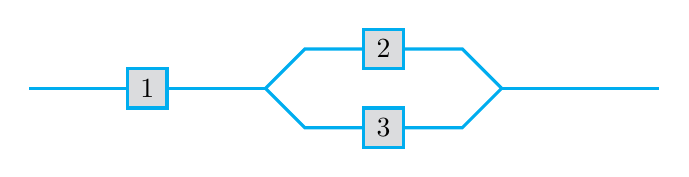
\begin{tikzpicture}[line width=0.4mm, draw=bookblue]
        \coordinate (A) at (3,0);
        \coordinate (B) at (3.5,0.5);
        \coordinate (C) at (5.5,0.5);
        \coordinate (D) at (6,0);
        \coordinate (E) at (5.5,-0.5);
        \coordinate (F) at (3.5,-0.5);

        \draw (0,0)--(A);
        \draw (A)--(B)--(C)--(D)--(E)--(F)--cycle;
        \draw (D)--(8,0);

        \filldraw[fill=bookgrey, draw=bookblue]
          (1.25,-0.25) rectangle (1.75,0.25)
          node[pos=.5] {1};

        \filldraw[fill=bookgrey, draw=bookblue]
          (4.25,0.25) rectangle (4.75,0.75)
          node[pos=.5] {2};

        \filldraw[fill=bookgrey, draw=bookblue]
          (4.25,-0.25) rectangle (4.75,-0.75)
          node[pos=.5] {3};
      \end{tikzpicture}
    \end{center}
    The experiment consists of determining the condition of each component [$S$ (success) for a functioning component and $F$ (failure) for a nonfunctioning component].
    \begin{enumerate}
      \item[a.]
        Which outcomes are contained in the event $A$ that exactly two out of the three components function?
        \begin{align*}
          A = \Set{SSF, SFS, FSS}
        \end{align*}
      \item[b.]
        Which outcomes are contained in the event $B$ that at least two of the components function?
        \begin{align*}
          B = \Set{SSF, SFS, FSS, SSS}
        \end{align*}
      \item[c.]
        Which outcomes are contained in the event $B$ that the system functions?
        \begin{align*}
          C = \Set{SSF, SFS, SSS}
        \end{align*}
        The system functions if and only if the first component functions and either the second or third component functions. Thus, the outcome must always start with $S$ and must end with at least one $S$ ($SS$, $SF$, or $FS$).
      \item[d.]
        List outcomes in $C^\prime$, $A \cup C$, $A \cap C$, $B \cup C$, and $B \cap C$.
        \begin{align*}
          C^\prime &= \Set{FFF, FSS, FSF, FFS} \\
          A \cup C &= \Set{SSF, SFS, SSS, FSS} \\
          A \cap C &= \Set{SSF, SFS} \\
          B \cup C &= B \\
          B \cap C &= C
        \end{align*}
        $C^\prime$ are the outcomes in which the system does not function. This is when component 1 fails and/or both components 2 and 3 fail.
        \\ \\
        $A \cup C$ is both sets combined, excluding duplicates. $A \cap C$ is the outcomes the sets have in common. $FSS$ is not in $B$ because the first component must not fail. $SSS$ is not in $A$ because it has more than 2 components functioning. Thus, these two outcomes are not in the intersection.
        \\ \\
        $B \cup C$ is $B$ because $C$ is a subset of $B$ (the system functioning requires at least 2 components to function). Thus, $C$ has no elements that $B$ doesn't already have. $B \cap C$ is $C$ because $C$ is a subset of $B$. Thus, $B$ contains all of $C$, so $C$ has every element in common wth $B$.
    \end{enumerate}
  \item[8.]
    An engineering construction firm is currently working on power plants at three different sites. Let $A_i$ denote the event that the plant at site $i$ is completed by the contract date. Use the operations of union, intersection, and complementation to describe each of the following events in terms of $A_1$, $A_2$, and $A_3$, draw a Venn diagram, and shade the region corresponding to each one.
    \begin{enumerate}
      \item[a.]
        At least one plant is completed by the contract date.
        \begin{align*}
          A_1 \cup A_2 \cup A_3
        \end{align*}
        \begin{center}
          \scalebox{0.5}{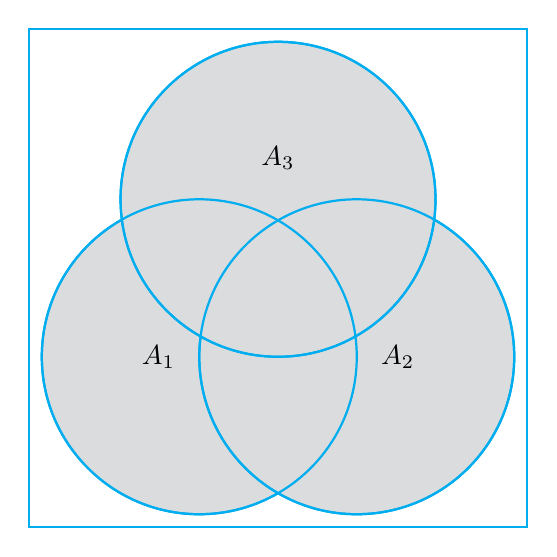
\begin{tikzpicture}[venn]
            \def\radius{2cm}

            \coordinate (A);
            \coordinate[xshift=\radius] (B);
            \coordinate[xshift=\radius / 2, yshift=\radius] (C);

            % Circles
            \draw[fill=bookgrey] (A) circle(\radius);
            \draw[fill=bookgrey] (B) circle(\radius);
            \draw[fill=bookgrey] (C) circle(\radius);

            % Redraw outlines without the fill
            % This fixes the fill overlapping outlines
            \draw (A) circle (\radius);
            \draw (B) circle (\radius);
            \draw (C) circle (\radius);

            % Labels
            \node[xshift=-0.5\radius] at (A) {$A_1$};
            \node[xshift=0.5\radius] at (B) {$A_2$};
            \node[yshift=0.5\radius] at (C) {$A_3$};
          \end{tikzpicture}}
        \end{center}
      \item[b.]
        All plants are completed by the contract date.
        \begin{align*}
          A_1 \cap A_2 \cap A_3
        \end{align*}
        \begin{center}
          \scalebox{0.5}{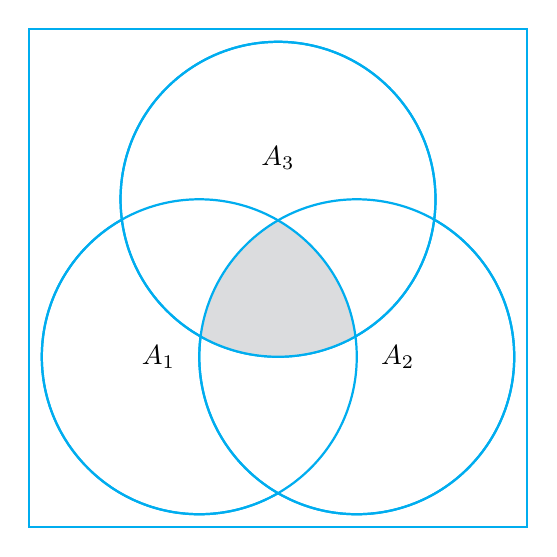
\begin{tikzpicture}[venn]
            \def\radius{2cm}

            \coordinate (A);
            \coordinate[xshift=\radius] (B);
            \coordinate[xshift=\radius / 2, yshift=\radius] (C);

            % Circles
            \draw[fill=white] (A) circle(\radius);
            \draw[fill=white] (B) circle(\radius);
            \draw[fill=white] (C) circle(\radius);

            % Intersection
            \begin{scope}[fill=bookgrey]
                \clip (A) circle(\radius);
                \clip (B) circle(\radius);
                \clip (C) circle(\radius);
                \fill (A) circle(\radius);
            \end{scope}

            % Redraw outlines without the fill
            % This fixes the fill overlapping outlines
            % It also fixes the clips not account for line thickness
            \draw (A) circle (\radius);
            \draw (B) circle (\radius);
            \draw (C) circle (\radius);

            % Labels
            \node[xshift=-0.5\radius] at (A) {$A_1$};
            \node[xshift=0.5\radius] at (B) {$A_2$};
            \node[yshift=0.5\radius] at (C) {$A_3$};
          \end{tikzpicture}}
        \end{center}
      \item[c.]
        Only the plant at site 1 is completed by the contract date.
        \begin{align*}
        A_ 1 \cap A_2^\prime \cap A_3^\prime
        \end{align*}
        \begin{center}
          \scalebox{0.5}{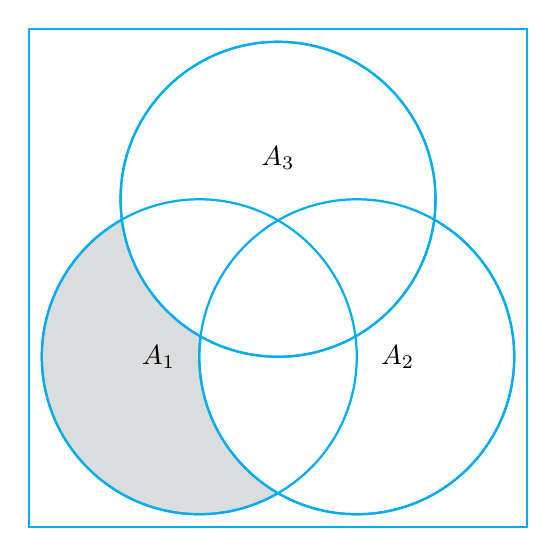
\begin{tikzpicture}[venn]
            \def\radius{2cm}

            \coordinate (A);
            \coordinate[xshift=\radius] (B);
            \coordinate[xshift=\radius / 2, yshift=\radius] (C);

            % Circles
            \draw[fill=bookgrey] (A) circle(\radius);
            \draw[fill=white] (B) circle(\radius);
            \draw[fill=white] (C) circle(\radius);


            % Redraw outlines without the fill
            % This fixes the fill overlapping outlines
            \draw (A) circle (\radius);
            \draw (B) circle (\radius);
            \draw (C) circle (\radius);

            % Labels
            \node[xshift=-0.5\radius] at (A) {$A_1$};
            \node[xshift=0.5\radius] at (B) {$A_2$};
            \node[yshift=0.5\radius] at (C) {$A_3$};
          \end{tikzpicture}}
        \end{center}
        Exclude the other sites by using their complements. Their intersection is used since it needs to be \textit{only} site 1.
      \item[d.]
        Exactly one plant is completed by the contract date.
        \begin{align*}
          (A_ 1 \cap A_2^\prime \cap A_3^\prime)
          \cup (A_ 1^\prime \cap A_2 \cap A_3^\prime)
          \cup (A_ 1^\prime \cap A_2^\prime \cap A_3)
        \end{align*}
        \begin{center}
          \scalebox{0.5}{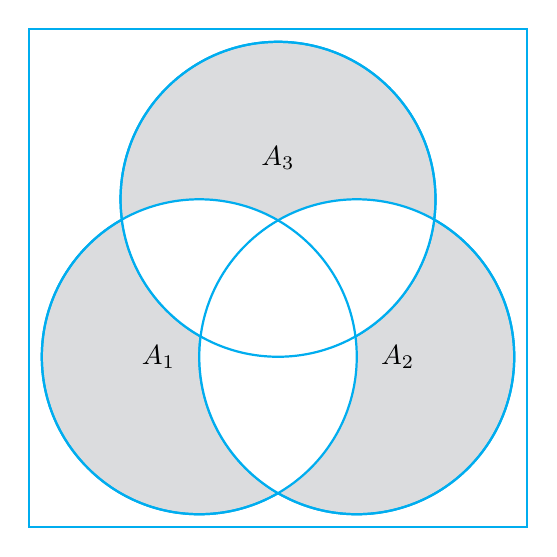
\begin{tikzpicture}[venn]
            \def\radius{2cm}

            \coordinate (A);
            \coordinate[xshift=\radius] (B);
            \coordinate[xshift=\radius / 2, yshift=\radius] (C);

            % Circles
            \draw[fill=bookgrey] (A) circle(\radius);
            \draw[fill=bookgrey] (B) circle(\radius);
            \draw[fill=bookgrey] (C) circle(\radius);

            % Intersection
            \begin{scope}[fill=white]
                \clip (A) circle(\radius);
                \clip (B) circle(\radius);
                \fill (0,0) circle(\radius);
            \end{scope}
           \begin{scope}[fill=white]
                \clip (C) circle(\radius);
                \fill (A) circle(\radius);
                \fill (B) circle(\radius);
            \end{scope}

            % Redraw outlines without the fill
            % This fixes the fill overlapping outlines
            % It also fixes the clips not account for line thickness
            \draw (A) circle (\radius);
            \draw (B) circle (\radius);
            \draw (C) circle (\radius);

            % Labels
            \node[xshift=-0.5\radius] at (A) {$A_1$};
            \node[xshift=0.5\radius] at (B) {$A_2$};
            \node[yshift=0.5\radius] at (C) {$A_3$};
          \end{tikzpicture}}
        \end{center}
        There are 3 sites, so 3 possible ways for exactly one plant to be completed. These are defined similar to (c). Since any of these 3 outcomes suffices, their union is used.
      \item[e.]
        Either the plant at site 1 or both of the other two plants are completed by the contract date.
        \begin{align*}
          (A_ 1 \cap A_2^\prime \cap A_3^\prime) \cup (A_ 1^\prime \cap A_2 \cap A_3)
        \end{align*}
        \begin{center}
          \scalebox{0.5}{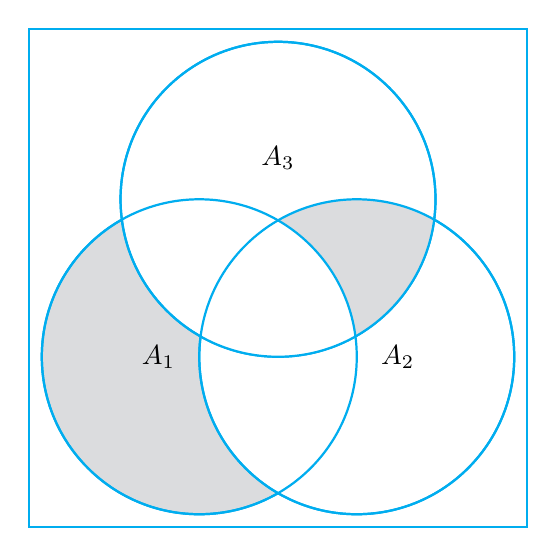
\begin{tikzpicture}[venn]
            \def\radius{2cm}

            \coordinate (A);
            \coordinate[xshift=\radius] (B);
            \coordinate[xshift=\radius / 2, yshift=\radius] (C);

            % Circles
            \draw[fill=bookgrey] (A) circle(\radius);
            \draw[fill=white] (B) circle(\radius);
            \draw[fill=white] (C) circle(\radius);

            % Intersection
            \begin{scope}[fill=bookgrey]
                \clip (B) circle(\radius);
                \fill (C) circle(\radius);
            \end{scope}
            \begin{scope}[fill=white]
                \clip (A) circle(\radius);
                \clip (B) circle(\radius);
                \clip (C) circle(\radius);
                \fill (A) circle(\radius);
            \end{scope}

            % Redraw outlines without the fill
            % This fixes the fill overlapping outlines
            % It also fixes the clips not account for line thickness
            \draw (A) circle (\radius);
            \draw (B) circle (\radius);
            \draw (C) circle (\radius);

            % Labels
            \node[xshift=-0.5\radius] at (A) {$A_1$};
            \node[xshift=0.5\radius] at (B) {$A_2$};
            \node[yshift=0.5\radius] at (C) {$A_3$};
          \end{tikzpicture}}
        \end{center}
        Only site 1 being complete was shown in (c). Only site 2 and 3 being completed is similar to (b), except $A$ has to be excluded by using its complement. As with (d), either of these two outcomes suffices, so their union is used.
    \end{enumerate}
\end{enumerate}

\end{document}
